\documentclass{article}
% \usepackage[utf8]{inputenc}
\usepackage{graphicx}
\graphicspath{ {images/} }
\usepackage{url}
\usepackage[T1]{fontenc} 


\title{\textbf{Transpiler For C To Python}}
\author{CS 252: Advanced Programming Languages \\
  Parth Jayantilal Jain \\
  San Jos\'{e} State University \\}
\begin{document}
\maketitle
\newpage
\begin{abstract}
There are many languages available to write a program for a computer. Many languages are domain specific. It is very difficult for a person to know all the languages. If a person knows the concept and knows the application then the programming language should not be a barrier. With this motivation i decided to implement a transpiler to convert a program given in C language to a program in Python.
\end{abstract}
\newpage
\tableofcontents

\newpage
\section{Introduction}
As there are so many programming languages available and this shouldn't be a barrier for implementing the ideas, I have implemented a transpiler in haskell to convert a C code to a python code. 
\subsection{What is Transpiler?}
A transpiler or source-to-source compiler, transcompiler is a type of compiler that takes
the source code of a program written in one programming language as its input and
produces the equivalent source code in another programming language.\cite{transpiler}
\subsection{Transpiler VS Compiler}
A transpiler translates between programming languages that operate at approximately
the same level of abstraction, while a traditional compiler translates from a higher level
programming language to a lower level programming language. For example, a
transpiler may perform a translation of a program from Python to C, whereas a compiler may perform a translation of a program from java to assembly language code.\cite{transpiler}
\subsection{Languages used}
A transpiler involves three languages, language for input program, language for output program, and the language in which the transpiler is used. In my project, the input program is in C language, the output program is in Python and the transpiler is written in haskell.

\newpage
\section{Features Supported}
\begin{itemize}
\item Main function
\item return 0
\item include statements
\item if loop
\item if loop with boolean operators (and, or, not)
\item while loop
\item while loop with boolean operators (and, or, not)
\item variable assignment (int, float, char)
\item arithmetic operations
\item support for relational operations
\item print string
\item print variables
\item increment
\item decrement
\item array initialization
\item open a file
\end{itemize}
\newpage

\section{Implementation}
The transpiler reads an input file and using parsec library from haskell parses the input file. Then using the concept of AST, i am doing pattern matching for the input program and then the appropriate python code is written to the output file.Now as we know there are no brackets used to describe the scope of a block in python. Python uses spacing or indentation for declaring the scope.Therefore, i wrote a python program to give indentation to the output code.
\\
I have included features for if loop and while loop, which can have one or two conditions, not more than that and these conditions are separated by either and operator, or operator or one condition consist of not operator. Both the loops can consist of multiple expressions inside the loop. Variables can be assigned an int value, a float value, a char, another variable, an arithmetic operation. The arithmetic operations supported are plus, minus, multiplication and division. It also has a feature of assigning an array with values, but all the values needs to be assigned at once. I have also added feature to open a file and handle main function. The program can consist of only one function that is the main function. I have also added features for handling relational operators, but only one operator can be used at a time. It also consist of features to print string and print variables. If you want to print a string and variable together, then the variable needs to be at the end of string. I have also added feature of increment and decrement operator.\cite{lecture} \\
\\
An example of C code:\\
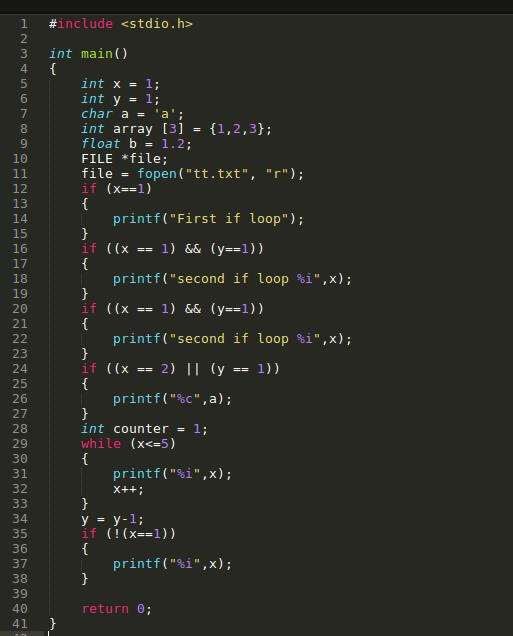
\includegraphics{la}

To run the transpiler, paste the file "project.hs" in the same folder as the input program. Open terminal and type the command runhaskell project.hs <inputfilename> > <outputfilename>. The outputfile should be a .txt file. Now paste the file indentation.py in the same folder as project.hs and now run the file indentation.py. The program will now ask for input filename, give .txt file generated by project.hs, then the program will ask for the output file, give the name of the output .py file. Now run the output python file.\\
\\
The final output file generated is:\\
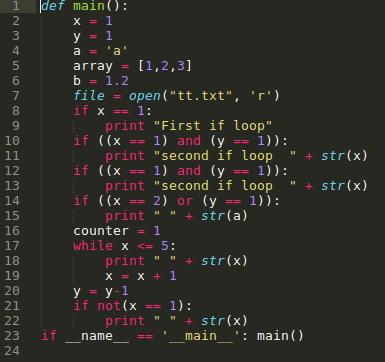
\includegraphics{la1}
\\
One of the challenges faced during adding feature for initializing variable with floating point value, was that if you parse the numbers after decimal using "many digit" or "many1 digit" then it is not able to identify zero. I solved this problem by parsing it in string format and separating the digits to the left and to right by using sepBy.


\section{Scope and Future Work}
In future, more features can be added like multiple arithmetic operations can be used in a single expression, loops can support more then two conditions. values of array can be accessed, and a particular value can be assigned to the array. Features to read, write and modify files can be added. The current version of transpiler supports some features and not the entire language, so more features can be added in future.

\section{Conclusion}
This project gave me an opportunity to learn how to design a transpiler, it also helped to understand the structure of the language design and how a compiler works. It also helped explore haskell language and its application.\

\bibliographystyle{plainurl}
\bibliography{ref.bib}
\end{document}
